\subsection{Optimization based on Local Search}
\label{subsec:localsearch}
\comment{
\noindent In this section we describe the construction of the tree. We split this process into the following two steps:
\begin{enumerate}
%\item {\bf {\em Constructing a similarity graph}}: We define a similarity metric for each pair of tags and threshold it appropriately to obtain a binary feature. i.e. we will call a tag pair {\bf {\em ``similar''}} iff their similarity score is greater than a threshold $t$. This is then used to build a similarity graph $\mathcal{G_t}$ where the vertices correspond to the tags and the edges correspond to tag pairs that are similar.
\item {\bf {\em Constructing a similarity graph}}: We start with the tree on the set of tags built using the WordNet database. We define a similarity metric for each pair of tags and threshold it appropriately to obtain a binary relation. i.e. we will call a tag pair {\bf {\em ``similar''}} iff their similarity score is greater than a threshold $t$. We then add the edges corresponding to similar tag pairs to the original tree and obtain the similarity graph which we will denote by $\mathcal{G_t}$.
\item {\bf {\em Building an optimized tree}}: On the set $\mathcal{S}$ of spanning trees of $\mathcal{G_t}$, we define a neighbour relation and a potential function and find a minimal tree using the local search paradigm.
\end{enumerate}

\subsection{Similarity Graph}

***** TODO (Chetan) ***** \\
--Fill in details of how initial tree using WordNet is constructed \\
********* \\



*****  TO BE FILLED **************** \\
-- Describe the threshold and the distribution from which it is calculated \\
--  We can't say $t$ is empirically estimated as mean $J(s_1, s_2)$ because that might make spanning trees infeasible \\
******************************************
}
Given the Similarity Graph $\mathcal{G_T}$ for a set of tags $\mathcal{T}$, our objective is to construct a spanning tree on $\mathcal{G_T}$ such that the defined objective function is minimized. Since finding spanning trees of $\mathcal{G_T}$ that optimally minimize either (\ref{eq:ObjFnWeightedHops}) or (\ref{eq:ObjFnSimApprox}) is a hard problem, we propose an approach to obtain local optimum through the local search paradigm. 
\\
\indent \textit{Local Search} -- Local search algorithms provide a local optimum to an optimization problem. This is done by moving from one solution to another, in the search space of candidate solutions. \\
For the problem of constructing a ontological tag tree, we define a simple edge-exchange based  neighborhood on the space of spanning trees of the graph $\mathcal{G_T}$ as follows. Given two spanning trees $T_1$, $T_2$ we say that $T_2$ is a neighbour of $T_1$ iff it can be obtained from $T_1$ by the following process:
\begin{enumerate}
	\item Pick an edge $e_1 \in \mathcal{G_T}\setminus T_1$ and add it to $T_1$. 
	\item In the (unique) cycle thus formed in $T_1$ containing $e_1$ pick the edge, say $e_2$ with minimum weight (i.e., jaccard similarity of the tags $e_2$ connects). Remove $e_2$ from $T_1$. 
\end{enumerate}
Starting from a spanning tree $T_0$ of $\mathcal{G_T}$ as an initial solution, we explore all neighbors of $T_0$ to determine which neighbor minimizes the defined objective function. The winning neighbor is then considered as the next solution and its neighbors are explored until no further benefit is seen in the objective function. The steps of the local search based ontological tree construction are listed in Algorithm~\ref{algo:STCAlgorithm}. The output is the locally optimal tag tree $T_{opt}$. Note that $T_0$ is taken as $T_W$ as obtained from Algorithm~\ref{alg:WordNetSTAlgo}. Fig.~\ref{fig:neighborhood} show one iteration of the proposed local search based approach for the objective function in (\ref{eq:ObjFnWeightedHops}). 
\begin{algorithm}
\fontsize{8pt}{1em}\selectfont
\caption{Ontological Tree Construction Algorithm}
\label{algo:STCAlgorithm} 
\textbf{Input:} \\
$\cdot$ Similarity graph $\mathcal{G_T}$ for a given set of tags $\mathcal{T}$ \\ 
$\cdot$ Initial Solution: $T_0$. \\
$\cdot$ \hl{Pair-wise Jaccard similarities between tags, i.e., $J_{\mathcal{T}}(i,j)$}
\textbf{Initialization:} 
$S$=$T_0$ \\
%$T_0$ can be randomly selected as any spanning tree over $\mathcal{G_T}$, or be picked in a heuristical manner \\
\textbf{Loop: } \\
\hspace*{5mm} $\cdot$ $E_{Candidates}$ := set of edges present in $\mathcal{G_T}$ and not in $S$ 
\hspace*{5mm} \textbf{For each edge $e$ in $E_{Candidates}$} \\
%\hspace*{10mm} (Exploring neighbors of current solution)  \\
\hspace*{10mm} $\cdot$ Add edge $e$ in $S$ to get graph $G$. \\
\hspace*{10mm} $\cdot$ $E_{Cycles}$ :=set of edges in the cycle formed in $G$. \\
\hspace*{10mm} $\cdot$ Remove edge $e'$ with lowest weight (i.e., jaccard \\
\hspace*{10mm} \; similarity of connecting tags) from $E_{Cycles}$: $e' \neq e$ \\
\hspace*{10mm} $\cdot$ $S_{Neighbor}$ = spanning tree thus formed  \\
\hspace*{10mm} $\cdot$ Calculate objective function at $S_{Neighbor}$ \\
\hspace*{5mm} \textbf{EndFor} \\
\hspace*{5mm} $\cdot$ Select neighbor giving best objective function as $S_{Next}$ \\
\hspace*{5mm} $\cdot$ If $S_{Next}$ improves objective function over $S$ \\
\hspace*{10mm} $S=S_{Next}$ \\
\hspace*{5mm} $\cdot$ Else Stop iterating \\ 
\textbf{End Loop}. \textbf{Output:} locally optimal spanning tree $T_{opt}=S$
\end{algorithm}

\begin{figure}[htbp]
\begin{center}
\centering
%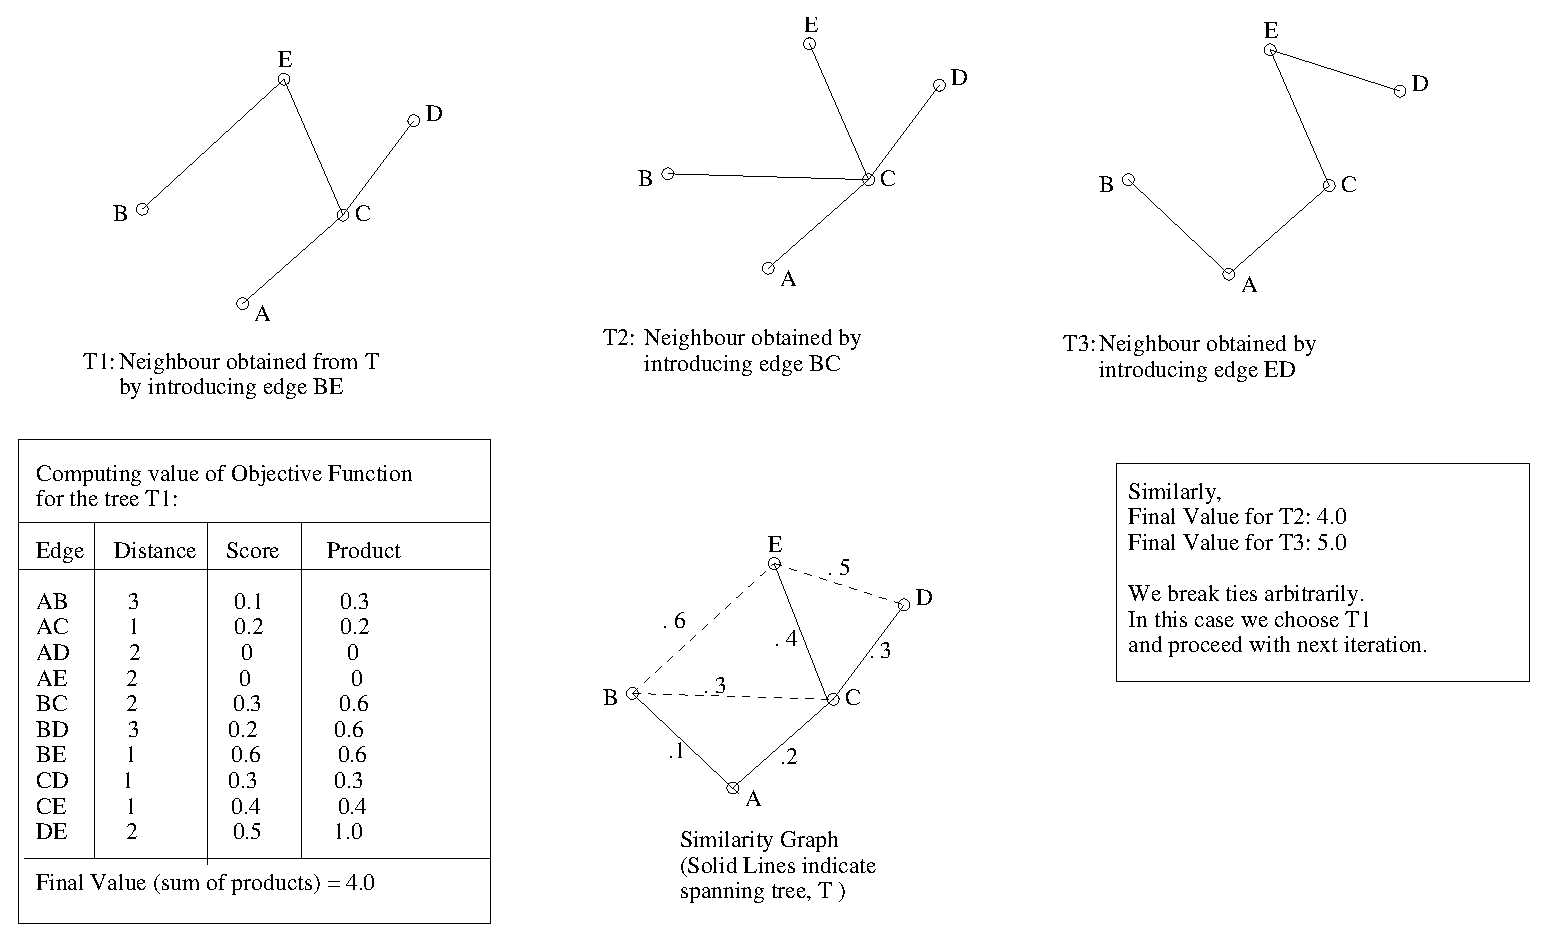
\includegraphics[width=0.8\linewidth]{Neighbourhood-2}
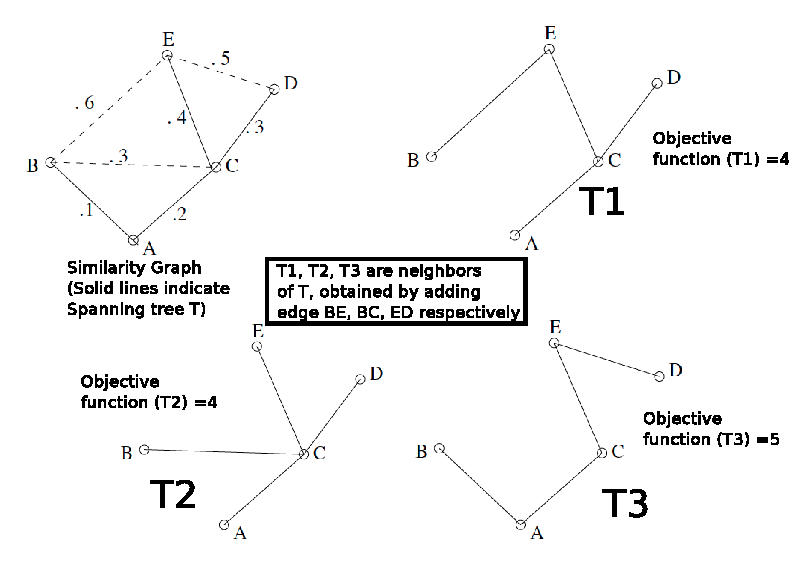
\includegraphics[width=0.8\linewidth]{TagTree/LSOneiteration}
\caption{One iteration of the proposed approach. Eq. (\ref{eq:ObjFnWeightedHops}) is utilized to calculate the objective function for neighbors of a tree T. Ties are broken arbitrarily. Since both T1 and T2 have an objective function~(\ref{eq:ObjFnWeightedHops}) value of 4, we choose T1 and proceed to next iteration. } 
\label{fig:neighborhood}
\end{center}
\end{figure}
% \subsubsection{Optimization Function} 
% \subsubsection{Local Search}
\subsection{Effect of initializing using WordNet}
\comment{
\hl{Utilizing a preliminary tag tree that is constructed using the semantics obtained WordNet has two benefits. Firstly, this biases the constructed structure to have connections dictated by semantic similarity when the data driven relations between certain tags are not strong enough to uniquely determine the structure of the tag tree. The constructed tag tree would thus have edges that are explicable based on the semantic similarity of the tags, as compared to randomness induced as an artefact of the construction procedure. As compared to other tag trees with possibly similar value of the objective function, the resulting tag trees offer a clean interpretation of the relationship between the tags. For example, consider four tags A, B, C, D with pair-wise jaccard similarities as given in Fig. {\ref{fig:ExampleWhyWordnet}}. 
}
\comment{
\begin{table}[htbp]
\scriptsize
\begin{center}
\caption{\hl{Example pair-wise jaccard similarities}}
\label{tab:ExampleWhyWordnet}
%\begin{tabular}{|p{4cm}|p{3.0cm}|}
\begin{tabular}{|c|c|c|c|c|}
		\hline
		 & A & B & C & D \\ 
		\hline 
		A & 1 & 0.9 & 0.1 & 0.3 \\ 
		\hline 
		 B & 0.9 & 1 & 0.2 & 0.2 \\ 
		\hline
		 C & 0.1 & 0.2 & 1 & 0.2 \\
		\hline
		D & 0.3 & 0.2 & 0.2 & 1 \\
		\hline 
\end{tabular}
\end{center}
\end{table}
}
\hl{Based on the first (LS-WAH) objective function ({\ref{eq:ObjFnWeightedHops}}), the two tag trees that would have the same value of the objective function (equal to 2.5) are shown in Fig.~{\ref{fig:whywordnet}} as X and Y. The tag tree as per WordNet is denoted by W. Random initializations of the local search based optimization as detailed in Section {\ref{sec:ConstructionTree}} can lead to either of X or Y as the solution. However initializing using W leads to a unique solution Y where tag B is connected to tags C and D, as in W, thus preferring connections that conform to their semantic relationship. \\
\textbf{Question: Should we even have the first para and its figs?\\ }
} }
\hl{The benefit of using WordNet to initialize the proposed local search based approach is that as compared to random initializations, the former helps achieve a preferred value of the objective function faster. The typical way to attain a lower value of the objective function for an optimization problem as defined in Section {\ref{sec:refinement}} would be to run the local search using randomly constructed tree on the set of tags as initialization, and picking the best tree across several such runs based on the tag tree that has lowest objective function. However this requires running the local search several times which can be large considering that the number of spanning trees on a set of $N$ tags varies as $N^{N-2}$~{\cite{cayley1894collected}}. The preliminary tree as constructed using WordNet offers a more meaningful initialization to the local search by capturing certain types of relationships between the tags that are dictated by their semantics. Table {\ref{tab:WordNetRandominitGWS30}} provides the statistics of the objective function of tag trees constructed by running the proposed local search based approach 20 times with random initializations. As can be seen, a single run using WordNet based preliminary tag tree leads to a much better objective function~({\ref{eq:ObjFnSimApprox}}). Also, the resulting tag tree using WordNet leads to a better performance than the best across 20 runs with random initializations. Note that for Table {\ref{tab:WordNetRandominitGWS30}}, the performance of tag trees is measured using Average Tag Prediction Accuracy as discussed in Section {\ref{sec:Expts}}.} 

\comment{
\begin{figure}[h]
\begin{center}
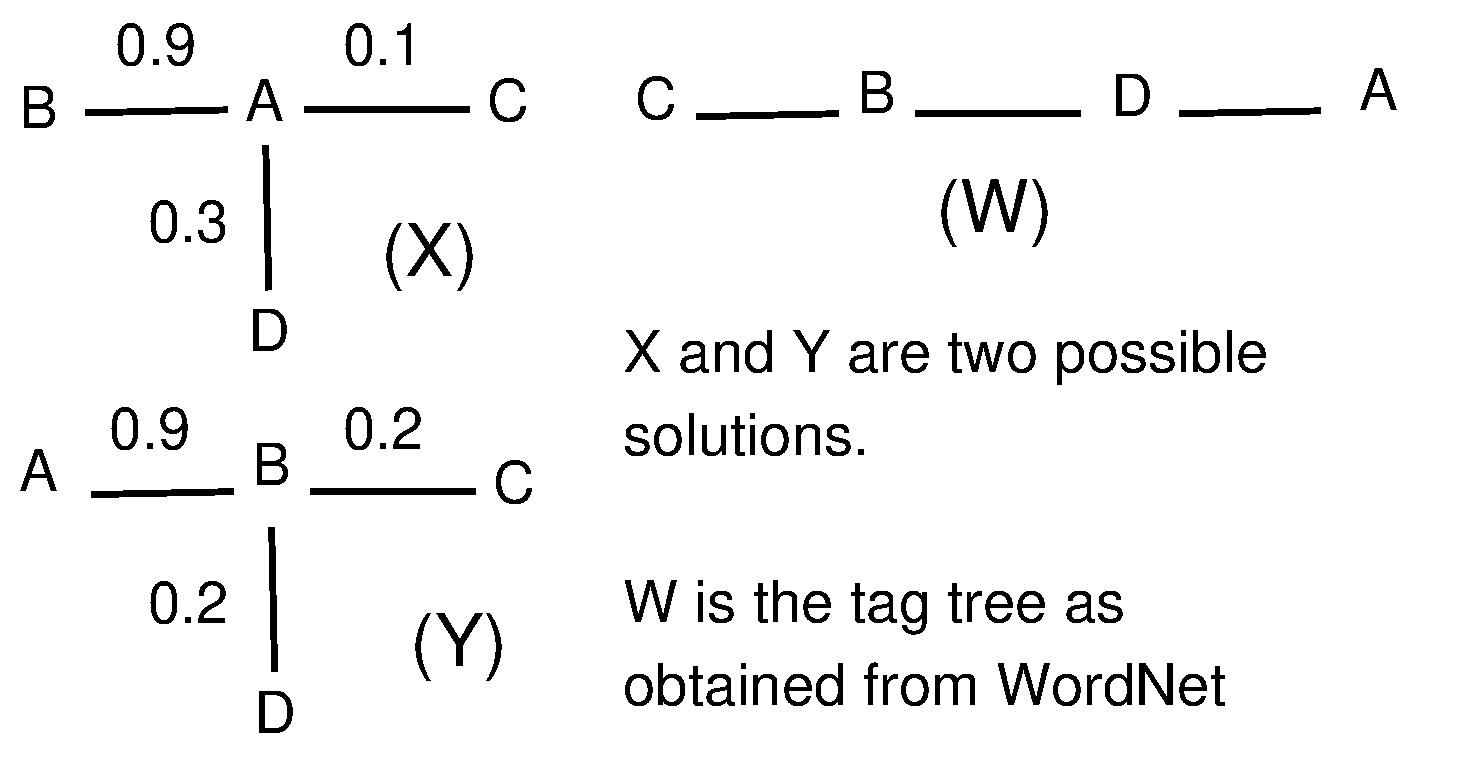
\includegraphics[width=0.65\linewidth]{TagTree/WhyWordNetExample}
\caption{\hl{Example showing multiple solutions using (LS-WAH) objective function ({\ref{eq:ObjFnWeightedHops}}) } }
\label{fig:whywordnet}
\end{center} 
\end{figure}
}
\comment{
\begin{figure}[t!]
\centering
\minipage{0.17\textwidth}
%\centering
  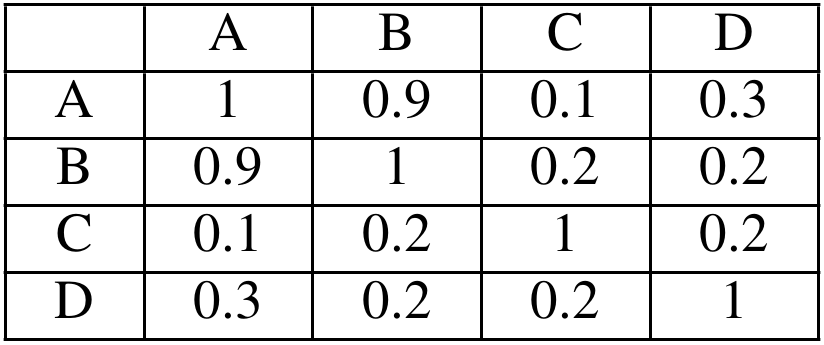
\includegraphics[width=\linewidth]{TagTree/TableWordNetExample.png} 
\caption{\hl{Example pair-wise jaccard similarities}}
\label{fig:ExampleWhyWordnet}
%\end{centering}
\endminipage %\hfill
\hspace{0.1in}
\minipage{0.28\textwidth}
  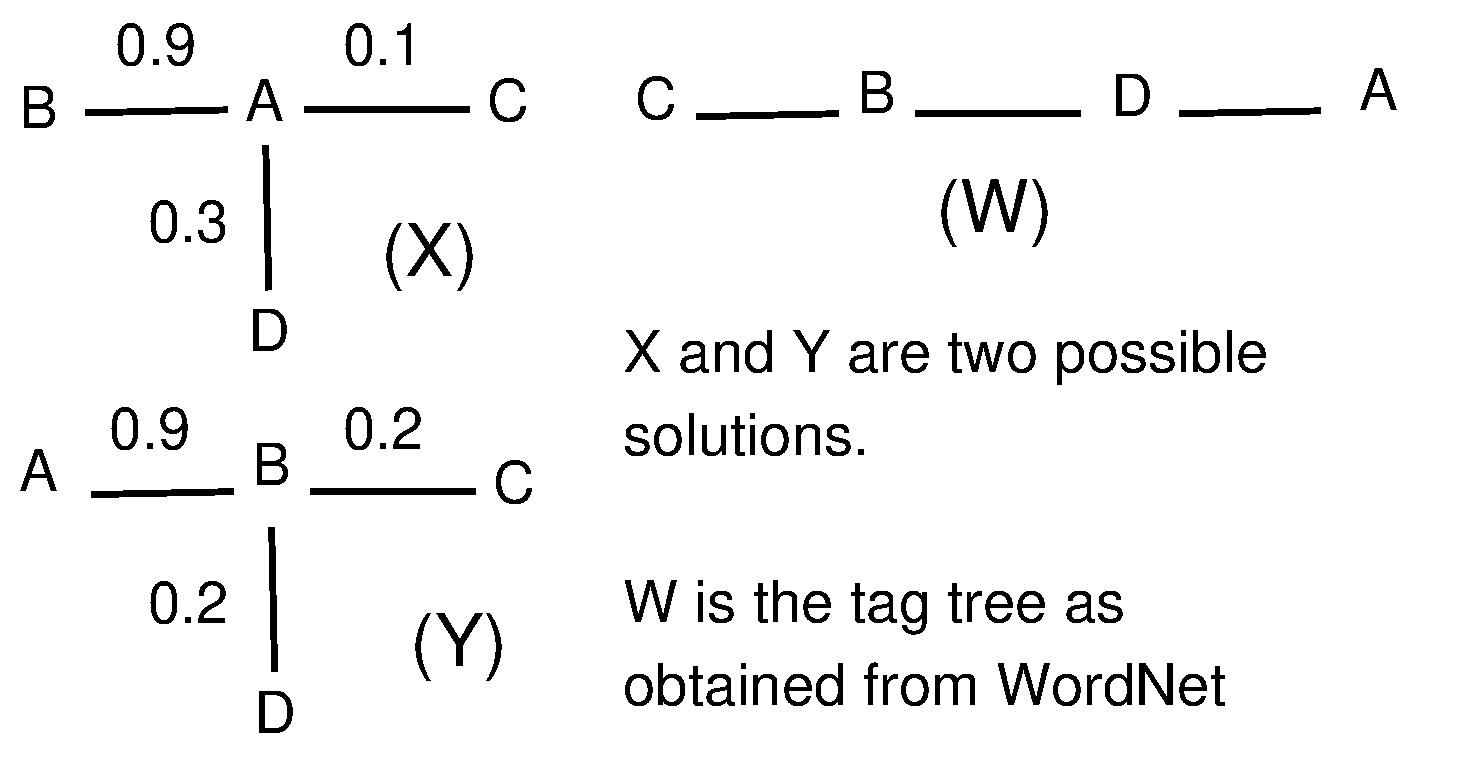
\includegraphics[width=\linewidth]{TagTree/WhyWordNetExample}
\caption{\hl{Example showing multiple solutions using (LS-WAH) objective function ({\ref{eq:ObjFnWeightedHops}}) } }
\label{fig:whywordnet}
\endminipage %\hfill
\end{figure}
}
\begin{table}[htbp]
%\scriptsize
\begin{center}
\caption{Effect of initializing the proposed local search based approach using WordNet. 30 tags from stock image corpus (described in Section IV) are used. }
\label{tab:WordNetRandominitGWS30}
\begin{tabular}{lllll}
\toprule 
     & \multicolumn{3}{c}{Random initialization} & \multicolumn{1}{c}{Using WordNet}\\

    & Min & Mean & Max & \multicolumn{1}{c}{}  \\
    \midrule
    Objective function ((4) x $10^6$) & 6.4    & 13.7  &  47.7  & \multicolumn{1}{c}{0.6} \\
    Performance (in \%) & 24.2    &43.8  & 49.2  & \multicolumn{1}{c}{50.9} \\
    \bottomrule
\end{tabular}
\end{center}
\end{table}